% Artículo del Proyecto Integrador (Producto de difusión)
% Basado en la plantilla oficial (articulo_plantilla.tex). Contenido transcrito sin cambios
% desde la vista previa; los marcadores pendientes se conservan resaltados con \pend{...}.
% Formato: carta, una columna, 11 pt, márgenes de 2.5 cm, interlineado 1.15.
% Compila con pdfLaTeX (opción predeterminada de Overleaf); no requiere Biber.
\documentclass[letterpaper,11pt]{article}

% --- Idioma y tipografía ---
\usepackage[T1]{fontenc}
\usepackage{lmodern}
\usepackage[spanish,es-tabla,es-nodecimaldot]{babel}

% --- Página: carta, márgenes 2.5 cm, interlineado 1.15 ---
\usepackage[margin=2.5cm]{geometry}
\geometry{headheight=52pt,headsep=0.3cm}
\usepackage{setspace}
\setstretch{1.15}

% --- Figuras y tablas ---
\usepackage{graphicx}
\usepackage{booktabs}
\usepackage{float}
\usepackage[font=small,labelfont=bf,labelsep=colon]{caption}
\usepackage{tabularx}
\usepackage{array}
\usepackage{enumitem}
\usepackage{amsmath}
\usepackage{xcolor}
\newcolumntype{L}{>{\raggedright\arraybackslash}X}

% --- Marcador de pendientes (resaltado amarillo, como en la vista previa) ---
\newcommand{\pend}[1]{\colorbox{yellow}{#1}}

% --- Encabezado: logo (logo.jpeg) solo en la primera página ---
\usepackage{fancyhdr}
\renewcommand{\headrulewidth}{0pt}
\fancypagestyle{plain}{%
  \fancyhf{}%
  \fancyhead[C]{
\includegraphics[height=1.2cm]{logo.jpeg}}%
  \fancyfoot[C]{\thepage}}
\pagestyle{fancy}
\fancyhf{}
\fancyfoot[C]{\thepage}

% --- Encabezados de sección ---
\usepackage{titlesec}
\titleformat{\section}{\Large\bfseries}{\thesection.}{0.6em}{}
\titleformat{\subsection}{\large\bfseries}{\thesubsection.}{0.6em}{}
\titlespacing*{\section}{0pt}{1.6ex plus 0.4ex minus 0.2ex}{1ex}

% --- Referencias: APA 7 ---
% Lista de referencias escrita en formato APA 7 al final del documento
% (sin biblatex/biber para reducir el tiempo de compilación en Overleaf).
\usepackage{xurl}

% --- Enlaces y URL (DOI); se carga al final ---
\usepackage[hidelinks]{hyperref}
\urlstyle{same}

% --- Título ---
\title{\textbf{Parada anticipada del MSAPSO frente a alternativas de aprendizaje y optimización para el seguimiento del punto de máxima potencia bajo sombreado parcial}}
\author{P. C. Márquez Correo, D. Molina León,\\[2pt]
  F. Moreira Guerra\\[6pt]
  \normalsize Proyecto Integrador · Maestría en Inteligencia Artificial Aplicada\\
  \normalsize Tecnológico de Monterrey\\[4pt]
  \normalsize Asesor: Prof. Gerardo J. Camacho González, PhD\\[4pt]
  \normalsize Equipo 53 -- Solar Optimization}
  

\begin{document}
\renewcommand{\abstractname}{Resumen}
\renewcommand{\tablename}{Tabla}
\renewcommand{\figurename}{Figura}

\maketitle

% --- Resumen (sin número) ---
\begin{abstract}
El seguimiento del punto de máxima potencia (MPPT) bajo sombreado parcial es difícil porque la curva potencia--corriente tiene varios máximos locales. Este trabajo exploratorio, sin fin comercial, parte del MSAPSO, un enjambre de siete partículas que usa 175 mediciones por búsqueda, y pregunta si es posible superarlo con aprendizaje por refuerzo, redes neuronales u optimización poblacional. Todas las versiones (V2 a V19) se compararon con el mismo simulador dinámico (convertidor Boost con control Super-Twisting), la energía entregada como métrica, intervalos de confianza bootstrap pareados, 2\,400 escenarios aleatorios y criterios fijados antes de cada corrida. Ninguna mejoró la exactitud final del MSAPSO, que ya está cerca de su techo, y varios éxitos iniciales desaparecieron al usar un baseline fiel. La única mejora que sobrevivió fue detener el enjambre cuando sus partículas se agrupan (V7): 70 mediciones en lugar de 175, 0.05~pp menos de exactitud, +2.78~pp de energía [IC 95\,\%: 2.39, 3.18] en 1\,200 escenarios de confirmación y una cola estática con p99 de 0.64~pp. La candidata con más energía (V14, +1.60~pp sobre la V7) tiene una cola de hasta 23~pp y no cumple el umbral previo de p99 $\leq$ 3~pp; al medir la cola con el límite de 12~$\Omega$ del convertidor cumple en el panel base (p99 de 1.4~pp), pero no en todos los paneles (hasta 6.4~pp). Dos variantes pedidas en la revisión del asesor, un MLP que recibe pares (corriente, potencia) y un DecentCEM con 10 muestras por iteración, bajan la cola pero pierden energía frente a la V7 ($-6.59$ y $-2.44$~pp). Concluimos que, con 40 a 70 mediciones, una condición de salida simple supera a modelos más complejos, que un margen del 2\,\% en la corriente es un hallazgo transferible y que la V7 es implementable tras validarse en hardware. Todos los resultados provienen de simulación.

\medskip
\noindent\textbf{Palabras clave:} MPPT, sombreado parcial, MSAPSO, parada anticipada, método de entropía cruzada, evaluación bajo cola de riesgo.
\end{abstract}

% =====================================================================
\section{Contexto de negocio y problema}

\subsection{El problema técnico}
Un panel fotovoltaico entrega su máxima potencia en un único punto de operación que cambia con la irradiancia y la temperatura. Cuando una parte del arreglo recibe menos luz por nubes, árboles o estructuras, la curva potencia--corriente deja de tener un solo máximo y aparecen varios máximos locales (Figura~\ref{fig:casos}). Los métodos clásicos de perturbar y observar o de conductancia incremental pueden quedarse en uno de ellos y no garantizan encontrar el máximo global (\textit{Hybrid MPPT with Deterministic PSO}, 2025). Cada medición cuesta tiempo, porque el convertidor debe asentarse en la corriente pedida; mientras el controlador busca, el panel entrega menos de lo que podría.

\begin{figure}[H]
  \centering
  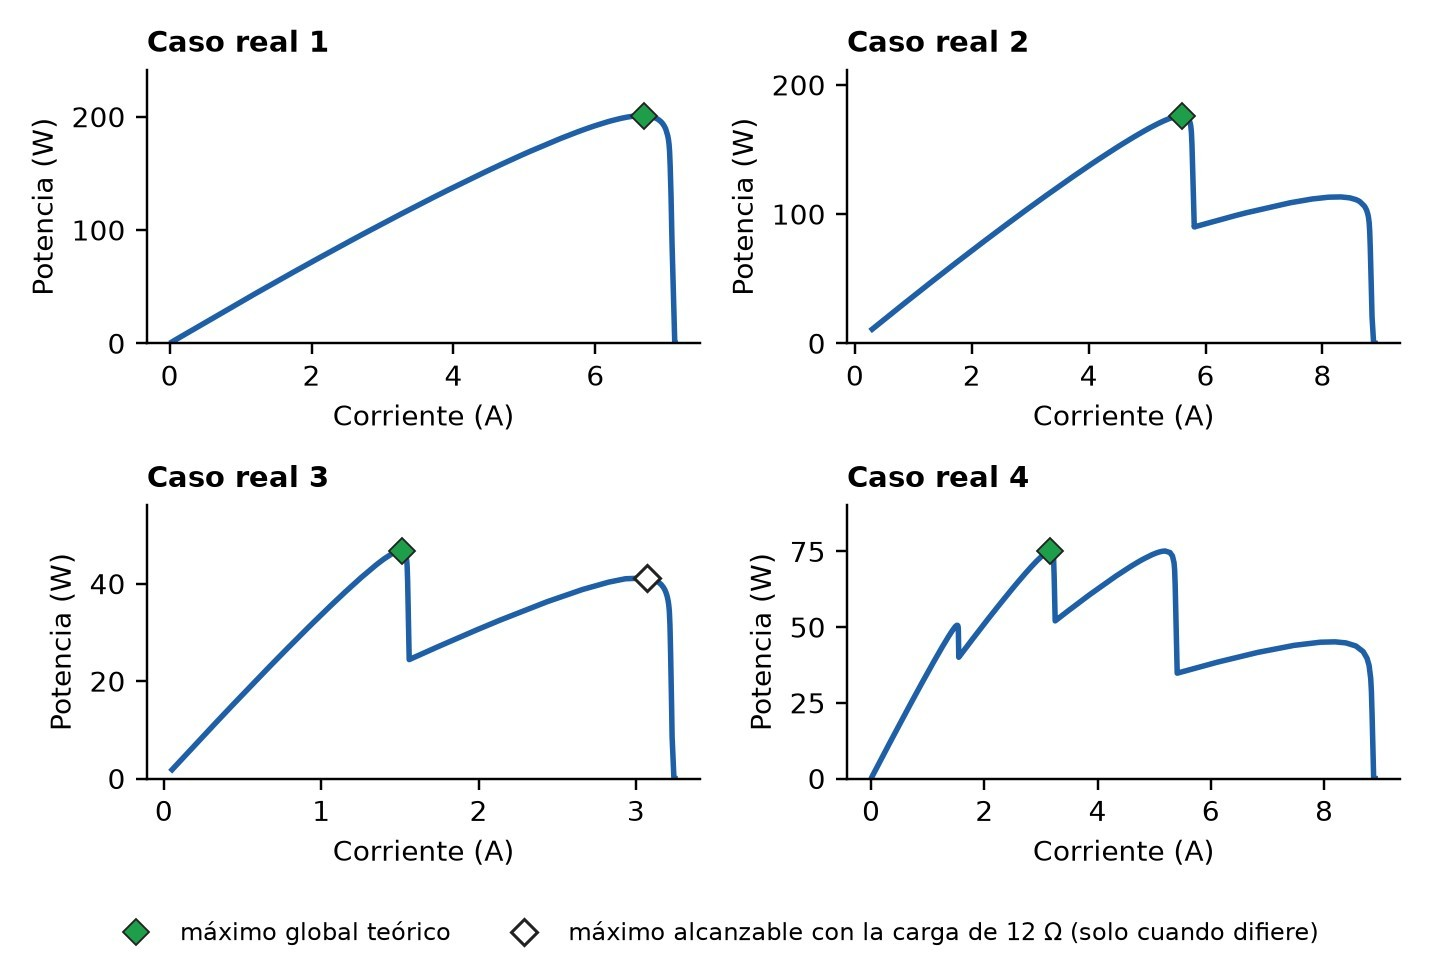
\includegraphics[width=0.82\linewidth]{figuras/fig1_casos_reales.jpg}
  \caption{Curvas potencia--corriente de los cuatro casos de referencia del manuscrito base. El Caso 1 es uniforme (un máximo); los casos 2 a 4 tienen sombra parcial con dos o tres máximos. En el Caso 3 el máximo global teórico (rombo verde) no es alcanzable con la carga de 12~$\Omega$; el máximo alcanzable se marca con el rombo vacío.}
  \label{fig:casos}
\end{figure}

El algoritmo de referencia es el MSAPSO, una variante determinista de la optimización por enjambre de partículas (Kennedy y Eberhart, 1995) descrita en el manuscrito base que proporcionó el asesor (\textit{Hybrid MPPT with Deterministic PSO}, 2025). Siete partículas se reparten en 0.95, 0.80, 0.65, 0.50, 0.30, 0.15 y 0.10 de la corriente de cortocircuito. En cada pasada se mide la potencia en las siete corrientes y cada partícula se acerca a la mejor posición encontrada con un factor $\beta$ que crece de 0.1 a 0.95 a lo largo de 25 pasadas, es decir, \textbf{175 mediciones por búsqueda}. Después fija la corriente del mejor punto y vuelve a buscar si la potencia cambia 5~W o más.

\subsection{Naturaleza del proyecto y valor esperado}
Este proyecto es una investigación exploratoria: no hay cliente, empresa ni fin comercial. El ``negocio'' es la eficiencia energética de los paneles: obtener más energía de la misma instalación, o la misma energía con menos tiempo y cómputo dedicados a buscar. En consecuencia, el valor no se mide en ingresos sino en energía entregada y en confiabilidad, de acuerdo con la recomendación de no fijar los indicadores alrededor del modelo mismo sino de resultados medibles y de ajustar la métrica a la madurez de la tecnología: para herramientas experimentales, medir si abren nuevas posibilidades de investigación (Korolov, 2022). Los interesados identificados son el asesor académico, el equipo de investigación y, de manera prospectiva, quienes operarían instalaciones con sombreado cambiante; como señala Miller (2022), un proyecto de inteligencia artificial involucra varios roles de interesados con responsabilidades distintas, que se retoman en la Sección~5.

\subsection{Enfoque adoptado y cambios de rumbo}
La pregunta inicial era si el aprendizaje por refuerzo podía mejorar al MSAPSO. Una primera versión (V1) parecía confirmarlo (de 82.9\,\% a 99.3\,\% de la potencia máxima), pero al re-validarla (V2) esa mejora resultó ser producto de la comparación y no del aprendizaje: el baseline no era el MSAPSO del manuscrito sino una versión más débil, la métrica (``mejor potencia encontrada'') no lo penalizaba y el agente recibía información que un controlador real no tendría (el máximo verdadero y el aviso de cambio de sombra). A partir de ahí el enfoque cambió de ``entrenar un modelo para reemplazar al MSAPSO'' a \textbf{buscar cualquier mejora verificable bajo una comparación justa}: el mismo simulador, la energía como métrica, varias semillas, intervalos de confianza y escenarios que no se usaron para elegir parámetros. Las líneas del asesor (políticas aprendidas, CEM, redes neuronales y optimización poblacional) se evaluaron bajo ese mismo protocolo.

\textbf{Pregunta de investigación:} ¿existe un método que supere al MSAPSO en energía entregada con menos mediciones, sin empeorar su exactitud ni su cola de riesgo?

\subsection{Umbrales de aceptación}
Antes de correr cada campaña se fijaron cuatro criterios para que un método reemplazara a la referencia vigente: \textbf{(a)} ventaja demostrable en energía, con intervalo de confianza de 95\,\% por encima de cero, tanto en el conjunto de prueba como en el de confirmación; \textbf{(b)} ninguna condición del desglose (panel, tiempo de espera, régimen de sombra, ruido) con una debilidad demostrable peor que $-1$~pp; \textbf{(c)} pérdida de más de 3~pp frente al MSAPSO en no más del 10\,\% de los escenarios; y \textbf{(d)} cola estática con pérdida media $\leq$ 0.5~pp y percentil 99 $\leq$ 3~pp. Los criterios (c) y (d) se centran en la cola porque una búsqueda que falla en una sombra persiste hasta que la sombra cambia.

% =====================================================================
\section{Datos y preparación}

\subsection{Fuentes de datos}
Se usaron dos fuentes. La primera son los \textbf{cuatro casos de referencia} del manuscrito base: curvas de un arreglo de cuatro subcadenas, con irradiancia uniforme en el Caso 1 (máximo teórico de 201.05~W) y combinaciones de 1\,000, 652, 607, 365 y 175~W/m² en los demás (Figura~\ref{fig:casos}). La segunda es un \textbf{generador de sombras sintéticas}: mezclas aleatorias de irradiancia por subcadena, con atenuación global opcional, evaluadas con el modelo de un diodo. No se dispone de mediciones en un sistema físico.

\subsection{Simulador dinámico}
La evaluación usa un convertidor Boost con inductor de 10~mH y carga resistiva de 12~$\Omega$, controlado por un algoritmo Super-Twisting (Levant, 2003). Una \textit{medición} es una ventana de duración t\_wait en la que el convertidor opera en la corriente pedida; el régimen de trabajo es 5~ms, porque a 0.5~ms el inductor no alcanza a seguir las referencias. Como el Boost solo puede presentar al panel puntos con $V/I \leq 12~\Omega$, el máximo teórico de la curva a veces es inalcanzable (Figura~\ref{fig:casos}, Caso 3); toda eficiencia se mide contra el \textbf{máximo alcanzable}, no contra el teórico.

\subsection{Diseño de escenarios y particiones}
Cada escenario es una secuencia de sombras (hasta 3\,000 ventanas) con un panel, un tiempo de espera, un régimen de cambio de sombra y un nivel de ruido muestreados con las frecuencias de la Tabla~\ref{tab:escenarios}. Las semillas son fijas (100000 + índice), de modo que todos los métodos ven exactamente los mismos escenarios. Los índices 600--1199 forman la partición de \textbf{ajuste}, la única que se usa para elegir parámetros; 0--599 son la \textbf{prueba} y 1200--2399 la \textbf{confirmación}, que nunca se usó para decidir nada. Como ningún método de búsqueda tiene pesos que se entrenen (salvo los MLP, que se entrenan con sombras aparte), su ``entrenamiento'' es este ajuste de parámetros.

\begin{table}[H]
  \centering
  \caption{Diseño de los 2\,400 escenarios. Cada escenario se muestrea de forma independiente con las probabilidades indicadas.}
  \label{tab:escenarios}
  \small
  \begin{tabularx}{\linewidth}{@{}p{3.4cm}L@{}}
    \toprule
    \textbf{Factor} & \textbf{Niveles (probabilidad)} \\
    \midrule
    Panel & base 60 celdas, 8.9~A (la de los casos de referencia del manuscrito); 72 celdas, 9.5~A; 36 celdas, 5.5~A; 60 celdas, 11~A; 96 celdas, 6.5~A (uniforme) \\
    Tiempo de espera & 5~ms (40\,\%); 2~ms (20\,\%); 1~ms (20\,\%); 0.5~ms (20\,\%) \\
    Régimen de sombra & único (30\,\%); moderado (15\,\%); alto (20\,\%); muy alto (10\,\%); parpadeo (20\,\%); estable (5\,\%) \\
    Ruido de medición & 0~W (50\,\%); 1~W (25\,\%); 2~W (25\,\%) \\
    Partición & ajuste 600--1199; prueba 0--599; confirmación 1200--2399 \\
    \bottomrule
  \end{tabularx}
\end{table}

\subsection{Preparación y calidad de los datos}
La posición de búsqueda se normaliza como $x = I/I_{sc}$, entre 0 y 1. Los modelos que se entrenan (políticas y redes neuronales) usan 30\,000 sombras sintéticas generadas con una semilla distinta de la de evaluación. Las limitaciones de datos que condicionan todo lo demás son cuatro. \textbf{(i) Todo es simulación}, y el MSAPSO es una reproducción propia a partir de la Fig.~6 de una versión borrador del manuscrito, no la implementación del autor. \textbf{(ii) Contaminación entre ajuste y evaluación:} la primera versión (V1) mostró que una comparación poco rigurosa infla los resultados, por eso el ajuste, la prueba y la confirmación se mantienen estrictamente separados. \textbf{(iii) Validez de las etiquetas y de las entradas:} las redes se entrenan con la corriente del máximo teórico, que puede ser inalcanzable con la carga fija; además, el MLP de la V11 se entrenó midiendo exactamente en las siete corrientes del barrido, mientras que en el convertidor las más bajas se miden en el borde de 12~$\Omega$. Con las potencias que realmente se miden, su error medio al ubicar el pico sube de 0.06 a 0.53 de $I_{sc}$. \textbf{(iv) Sin corrección por comparaciones múltiples}, de modo que la selección entre decenas de configuraciones sesga a favor de lo seleccionado; por eso la confirmación se reserva al final.

% =====================================================================
\section{Metodología y modelos}

\subsection{Baseline y protocolo de evaluación}
El baseline es el \textbf{MSAPSO del manuscrito} con sus parámetros originales (175 mediciones fijas). La métrica primaria es la \textbf{energía entregada} durante todo el escenario, expresada como porcentaje de la energía que se habría entregado operando siempre en el máximo alcanzable; incluye la inercia del convertidor, el tiempo perdido buscando y los reinicios. Las diferencias entre métodos se reportan en puntos porcentuales (pp) con intervalos de confianza de 95\,\% por bootstrap pareado sobre los escenarios (3\,000 remuestreos; Efron y Tibshirani, 1993). Como métrica secundaria se mide la \textbf{cola estática}: en 1\,000 curvas de sombra con una sola búsqueda, la pérdida de exactitud final frente al MSAPSO (media, percentil 99 y máximo). Se reporta de dos formas. La \textbf{cola oficial} mide la potencia en cualquier corriente pedida y compara contra el máximo teórico. La \textbf{cola con borde de 12~$\Omega$}, añadida en la revisión del asesor, mide en el borde lo que se pide en la zona que el Boost no alcanza y compara contra el máximo alcanzable, como ocurre en el simulador dinámico. La segunda no penaliza a un método por no encontrar un pico que el convertidor nunca podría usar.

\subsection{Recorrido de las versiones}
El trabajo avanzó en cinco etapas, que corresponden a los avances del proyecto situado en el periodo académico de septiembre a diciembre de la Maestría en Inteligencia Artificial Aplicada que se dicta de forma virtual por el Tecnológico de Monterrey, más una revisión final pedida por el asesor. La Tabla~\ref{tab:recorrido} resume lo que se probó en cada una, lo que se encontró y qué se decidió. Las políticas aprendidas usaron REINFORCE (Williams, 1992) y PPO (Schulman et al., 2017); el método de entropía cruzada (CEM) sigue a Rubinstein y Kroese (2004).

\begin{table}[H]
  \centering
  \caption{Recorrido del proyecto por etapas (Avances 1 a 5). pp = puntos porcentuales de energía. Las cifras de cada versión proceden de su reporte (Anexo~A).}
  \label{tab:recorrido}
  \footnotesize
  \setstretch{1}
  \begin{tabularx}{\linewidth}{@{}p{1.55cm}p{4.1cm}Lp{2.9cm}@{}}
    \toprule
    \textbf{Etapa y versiones} & \textbf{Qué se probó} & \textbf{Hallazgo} & \textbf{Decisión} \\
    \midrule
    \textbf{Avance 1} V2 & Re-validación del primer resultado con simulador compilado, MSAPSO fiel a la Fig.~6, sin información filtrada al agente, PPO, A2C, SAC y REINFORCE, 3 semillas. & La ``mejora'' previa (82.9 $\rightarrow$ 99.3\,\%) venía del baseline débil y de la información filtrada, no del aprendizaje. PPO gana +1.84~pp en sombra estática, pero una regla simple sin aprendizaje lo iguala. & Baseline fiel, energía como métrica; régimen de 5~ms. \\
    \addlinespace
    \textbf{Avance 2} V4--V6 & Esquema del asesor: potencias medidas $\rightarrow$ MLP con política gaussiana (V4); correcciones del objetivo, PPO, SAC, DDPG y árbol de decisión (V5); híbrido ``el modelo ubica, el MSAPSO afina'' (V6). & No superan a un control simple (V4). Con pocas mediciones ganan $\approx$ 3~pp (V5) pero quedan 1--2~pp bajo el MSAPSO en exactitud. El híbrido gana +3~pp en estático con 6$\times$ menos mediciones y pierde $\approx$ 3~pp en dinámico con sombras sintéticas (V6). & El MSAPSO se mantiene como base. \\
    \addlinespace
    \textbf{Avance 3} V7--V9 & V7: parada anticipada del MSAPSO. V8: parada aprendida con un árbol sobre 13 señales. V9: memoria de patrones de sombra. & V7: 175 $\rightarrow$ 70 mediciones con $-0.05$~pp de exactitud; +3.0~pp [2.7, 3.3] en 2\,400 escenarios. V8 no mejora la regla simple. V9 acierta solo en 3--15\,\% de los casos dinámicos. & \textbf{V7 = método principal.} \\
    \addlinespace
    \textbf{Avance 4} V10--V14 & CEM puro (V10); MLP supervisado + CEM (V11); MSAPSO corto + CEM (V12); retroceso del 2\,\% (V13); campaña completa (V14). & CEM puro pierde exactitud y colapsa su $\sigma$. El retroceso del 2\,\% reproduce la ventaja dinámica del MLP sin entrenar. La candidata V14 gana +1.54~pp [1.31, 1.78] sobre la V7 pero con cola p99 de 13~pp. & V14 no cumple (d); el retroceso queda como hallazgo. \\
    \addlinespace
    \textbf{Avance 5} V15--V19 & DGBCO (V15); DGO/CEDGO (V16); DecentCEM con $\sigma$ fija (V17); MLP con corrientes como entrada (V18); demostración interactiva (V19). & Con 40 a 70 mediciones, ninguno supera a la V7 con cola aceptable. DecentCEM baja la cola de la V14 (p99 de 13 a 5.3~pp) pero no gana energía de forma demostrable. Las corrientes ayudan al MLP solo con puntos aleatorios (+0.74~pp). & La V7 se mantiene. \\
    \addlinespace
    \textbf{Revisión del asesor} & Cola con borde de 12~$\Omega$; MLP + CEM con pares (I, P) entrenado con el borde; DecentCEM 10$\times$4 (10 muestras por iteración, \% de élites de 10 a 100); tabla de ajuste, prueba y confirmación; simulador interactivo. & Con borde, la V14 cumple la cola en el panel base (p99 1.4~pp) pero no en todos los paneles (hasta 6.4~pp). El MLP con pares baja su cola con borde (15.3 $\rightarrow$ 6.9~pp) y pierde $-6.59$~pp en dinámica. El DecentCEM 10$\times$4 cumple la cola (p99 1.3~pp) pero pierde $-2.44$~pp. Sin sobreajuste entre particiones. & La V7 se mantiene; la V14 queda como alternativa con condiciones. \\
    \bottomrule
  \end{tabularx}
\end{table}

\subsection{La decisión que importó}
De todo lo hecho, una decisión explica el resultado: \textbf{cambiar la forma de evaluar}. En lugar de comparar exactitud final en pocas curvas estáticas, se pasó a medir energía entregada en un simulador dinámico, sobre miles de escenarios aleatorios, con criterios y particiones fijados antes de correr y mirando explícitamente la cola. Esa decisión tuvo tres consecuencias. Primero, hizo desaparecer éxitos que parecían sólidos (la mejora de la V1, el esquema de políticas de la V4, el híbrido de la V6). Segundo, mostró que el margen sobre el MSAPSO no está en la exactitud final, sino en el costo de búsqueda y en la energía con sombra cambiante. Tercero, reveló una \textbf{cola de riesgo} que las pruebas pequeñas ocultaban: varios métodos ganaban energía media, pero fallaban gravemente en el peor caso.

\subsection{Modelo final: MSAPSO con parada anticipada (V7)}
La V7 no cambia el MSAPSO; solo cambia \textbf{cuándo deja de buscar}. Después de cada pasada (mínimo tres) calcula la dispersión del enjambre, std($x$)/$I_{sc}$, y se detiene cuando es menor que 0.02, es decir, cuando las partículas ya se agruparon. No requiere entrenamiento, tiene unas 30 operaciones por pasada y conserva la regla de reinicio de 5~W. Se estudiaron reglas alternativas de reinicio y de parada y ninguna mejoró esta configuración, que además es estable ante variaciones de sus parámetros (solo son peligrosos t\_max $\leq$ 15 o umbrales $\geq$ 0.03). Los otros diez métodos comparados (Anexo~B) se evaluaron con la configuración congelada de su propia campaña, sin reajustes posteriores.

Los once métodos comparados son, en una frase cada uno: el \textbf{MSAPSO} de referencia; la \textbf{V7}, que lo detiene al converger; la \textbf{V7 con retroceso}, que opera al 98\,\% de la corriente hallada; el \textbf{CEM puro}, una gaussiana sobre la corriente que se reajusta con sus mejores muestras; el \textbf{MLP + CEM}, donde una red entrenada ubica el pico y el CEM lo refina; el \textbf{MLP + CEM con pares (I, P)}, la misma idea con una red que recibe la corriente medida junto con cada potencia y que se entrenó con el borde de 12~$\Omega$; la \textbf{candidata V14}, tres pasadas del enjambre más CEM más retroceso; \textbf{DGBCO}, agentes divididos en grupos de exploración y explotación (Moosavi et al., 2022); \textbf{CEDGO}, grupos con cabeza y entropía cruzada (Tang et al., 2017); y \textbf{DecentCEM}, que mide puntos repartidos, separa los máximos y refina cada uno con su propia gaussiana de $\sigma$ fija (Zhang et al., 2022; Moss, 2020); y el \textbf{DecentCEM 10$\times$4}, el mismo con 10 muestras por iteración en lugar de 4 y un porcentaje de élites ajustable, del que se reporta el 10\,\% elegido en el ajuste.

% =====================================================================
\section{Resultados y validación}

\subsection{El modelo final frente al baseline}
En los 1\,200 escenarios de confirmación la V7 entrega \textbf{87.38\,\%} de la energía máxima alcanzable contra 84.60\,\% del MSAPSO, es decir, una mejora de \textbf{+2.78~pp} [IC 95\,\%: 2.39, 3.18], equivalente a un aumento relativo de 3.3\,\%. En la prueba (0--599) es +2.98~pp [2.47, 3.50]. Usa 70 mediciones en lugar de 175 ($-60$\,\%) y pierde solo 0.05~pp de exactitud final. La ventaja es consistente: es positiva en los cinco paneles (de +2.1 a +4.1~pp), en los cuatro tiempos de espera (de +2.4 a +3.5~pp) y en los tres niveles de ruido (de +1.6 a +3.3~pp). Se concentra donde la sombra cambia con frecuencia (régimen alto +6.7~pp, muy alto +6.3~pp, moderado +3.1~pp, parpadeo +2.0~pp); con cambio aislado ($-0.2$~pp) o sombra estable ($-1.2$~pp) no hay ganancia.

\begin{table}[H]
  \centering
  \caption{Los once métodos con el mismo protocolo. Energía: 1\,200 escenarios de confirmación (diferencia en pp, IC 95\,\%). Cola estática: 1\,000 curvas; pérdida de exactitud frente al MSAPSO, oficial y con borde de 12~$\Omega$. Med.: mediciones promedio por búsqueda en esas curvas (cola oficial).}
  \label{tab:metodos}
  \scriptsize
  \setstretch{1}
  \setlength{\tabcolsep}{2.6pt}
  \resizebox{\linewidth}{!}{%
  \begin{tabular}{@{}lrllrrrrrrr@{}}
    \toprule
     & & & & & \multicolumn{3}{c}{\textbf{Cola oficial}} & \multicolumn{3}{c}{\textbf{Cola con borde 12~$\Omega$}} \\
    \cmidrule(lr){6-8}\cmidrule(l){9-11}
    \textbf{Método} & \textbf{Med.} & \textbf{Energía vs MSAPSO} & \textbf{Energía vs V7} & \textbf{$>$3 pp} & \textbf{media} & \textbf{p99} & \textbf{máx.} & \textbf{media} & \textbf{p99} & \textbf{máx.} \\
    \midrule
    MSAPSO del paper (base) & 175 & --- & $-2.78$ [$-3.18$, $-2.39$] & --- & --- & --- & --- & --- & --- & --- \\
    \textbf{V7 parada anticipada} & 70 & \textbf{+2.78} [2.39, 3.18] & --- & 8\,\% & 0.05 & 0.64 & 0.97 & 0.03 & 0.27 & 0.64 \\
    V7 + retroceso 2\,\% & 70 & +3.14 [2.73, 3.54] & +0.35 [0.15, 0.56] & 9\,\% & 0.53 & 1.79 & 2.26 & 0.41 & 1.11 & 1.70 \\
    Candidata V14 & 39 & +4.38 [3.95, 4.82] & +1.60 [1.24, 1.96] & 7\,\% & 0.88 & 13.0 & 23.0 & 0.45 & 1.38 & 6.31 \\
    MLP + CEM (V11) & 37 & +3.80 [3.19, 4.39] & +1.01 [0.49, 1.50] & 18\,\% & 0.82 & 11.7 & 21.3 & 2.74 & 15.3 & 20.4 \\
    MLP + CEM con pares (I, P) & 37 & $-3.81$ [$-4.57$, $-2.98$] & $-6.59$ [$-7.36$, $-5.82$] & 40\,\% & 1.32 & 17.6 & 29.5 & 0.40 & 6.94 & 10.2 \\
    DecentCEM (V17) & 40 & +3.13 [2.59, 3.65] & +0.35 [$-0.11$, 0.79] & 17\,\% & 0.25 & 5.3 & 7.6 & 0.19 & 4.00 & 9.43 \\
    DecentCEM 10$\times$4 (10\,\% élites) & 85 & +0.35 [$-0.20$, 0.89] & $-2.44$ [$-2.92$, $-1.96$] & 28\,\% & 0.02 & 1.33 & 7.22 & 0.07 & 2.52 & 9.43 \\
    DGBCO (V15) & 40 & +3.64 [3.13, 4.13] & +0.85 [0.47, 1.22] & 16\,\% & 2.26 & 15.9 & 25.1 & 1.43 & 11.3 & 18.6 \\
    CEM puro (V10) & 59 & +1.52 [0.96, 2.09] & $-1.26$ [$-1.78$, $-0.77$] & 22\,\% & 1.35 & 20.1 & 36.6 & 1.18 & 13.4 & 21.1 \\
    CEDGO (V16) & 41 & +1.98 [1.39, 2.54] & $-0.81$ [$-1.32$, $-0.31$] & 22\,\% & 3.36 & 28.9 & 59.2 & 2.61 & 26.9 & 43.5 \\
    \bottomrule
  \end{tabular}}
  \par\smallskip\raggedright\scriptsize $>$3 pp: porcentaje de escenarios dinámicos en que el método pierde más de 3~pp de energía frente al MSAPSO. Las colas con borde de la V7 + retroceso, la V14 y el DGBCO son una réplica propia sobre las mismas curvas y pueden diferir en décimas.
\end{table}

\begin{table}[H]
  \centering
  \caption{Ventaja de la V7 sobre el MSAPSO por condición, en los 1\,200 escenarios de confirmación (diferencia de energía en pp, IC 95\,\%). Ventaja demostrable cuando el intervalo queda por encima de cero.}
  \label{tab:condicion}
  \small
  \setstretch{1}
  \begin{tabular}{@{}llrrcc@{}}
    \toprule
    \textbf{Factor} & \textbf{Nivel} & \textbf{n} & \textbf{Diferencia} & \textbf{IC 95\,\%} & \textbf{¿Ventaja demostrable?} \\
    \midrule
    Régimen de sombra & muy alto & 126 & +6.34 & [+5.28, +7.41] & Sí \\
     & alto & 236 & +6.66 & [+5.67, +7.71] & Sí \\
     & moderado & 183 & +3.08 & [+1.93, +4.25] & Sí \\
     & parpadeo & 273 & +1.97 & [+1.46, +2.50] & Sí \\
     & único & 336 & $-0.22$ & [$-0.74$, +0.26] & Indeterminado \\
     & estable & 46 & $-1.23$ & [$-4.65$, +1.33] & Indeterminado \\
    \addlinespace
    Tiempo de espera & 0.5 ms & 240 & +3.46 & [+2.50, +4.41] & Sí \\
     & 1 ms & 250 & +2.91 & [+1.96, +3.79] & Sí \\
     & 2 ms & 248 & +2.68 & [+1.88, +3.49] & Sí \\
     & 5 ms & 462 & +2.41 & [+1.82, +3.00] & Sí \\
    \addlinespace
    Panel & base & 244 & +2.64 & [+1.90, +3.41] & Sí \\
     & 72c-6s & 212 & +2.11 & [+1.13, +2.97] & Sí \\
     & 36c-3s & 260 & +2.31 & [+1.50, +3.18] & Sí \\
     & 60c-11A & 233 & +2.66 & [+1.71, +3.60] & Sí \\
     & 96c-6.5A & 251 & +4.09 & [+3.18, +5.01] & Sí \\
    \addlinespace
    Ruido & 0 W & 611 & +3.29 & [+2.73, +3.86] & Sí \\
     & 1 W & 315 & +2.83 & [+1.98, +3.70] & Sí \\
     & 2 W & 274 & +1.59 & [+0.93, +2.24] & Sí \\
    \bottomrule
  \end{tabular}
\end{table}

La Tabla~\ref{tab:condicion} muestra que la ventaja se concentra en los regímenes de sombra que cambian con frecuencia y que, en sombra estable o de cambio aislado, la V7 no mejora al MSAPSO: es una condición de uso: con sombra estable o de cambio aislado hay pocas búsquedas que acelerar, así que no hay ganancia y aparece algo de varianza. La ventaja también es menor con ruido alto (2~W), posiblemente porque la regla de parada se basa en la dispersión del enjambre, que el ruido perturba (esta explicación no se aisló en un experimento).

\subsection{Comparación con los candidatos y cumplimiento de los umbrales}
La Figura~\ref{fig:energia} y la Tabla~\ref{tab:metodos} muestran que casi todo lo que se probó supera al MSAPSO en energía, porque el MSAPSO gasta 175 mediciones en cada búsqueda. La pregunta relevante es si algo supera a la V7. Cuatro métodos lo hacen con intervalo por encima de cero en la confirmación: la candidata V14 (+1.60~pp), el MLP + CEM (+1.01), DGBCO (+0.85) y el retroceso del 2\,\% sobre la V7 (+0.35). Los otros cinco (CEM puro, CEDGO, DecentCEM y las dos variantes de la revisión) empatan o pierden. Las dos variantes nuevas son las únicas que no superan con claridad ni siquiera al MSAPSO: el MLP con pares pierde $-3.81$~pp frente a él, sobre todo con esperas cortas ($-18$~pp frente a la V7 con 0.5~ms), porque la corriente medida va rezagada respecto de la pedida y la red recibe pares que no vio al entrenar; el DecentCEM 10$\times$4 empata con el MSAPSO (+0.35~pp [$-0.20$, 0.89]) porque usa unas 85 mediciones por búsqueda en lugar de 40.

\begin{figure}[H]
  \centering
  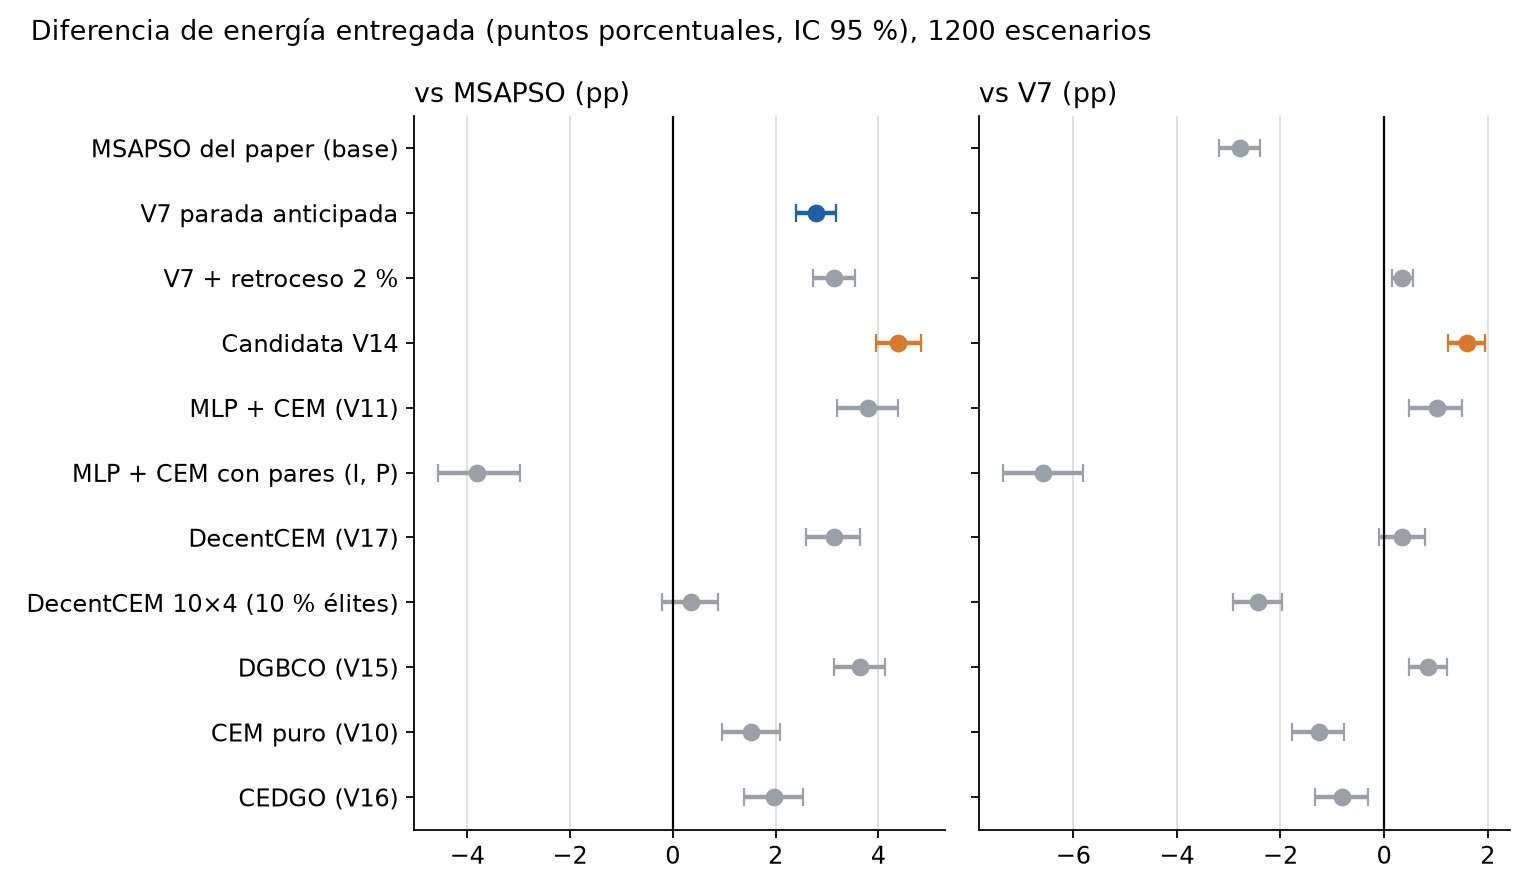
\includegraphics[width=0.82\linewidth]{figuras/fig2_energia.jpg}
  \caption{Diferencia de energía entregada de cada uno de los once métodos frente al MSAPSO (izquierda) y frente a la V7 (derecha), con intervalos de confianza de 95\,\% sobre 1\,200 escenarios de confirmación. Se resalta la V7 (azul) y la candidata V14 (naranja).}
  \label{fig:energia}
\end{figure}

Sin embargo, ganar energía media no basta. La Figura~\ref{fig:cola} coloca cada método según su energía frente a la V7 y su cola estática, con las dos medidas de cola. Con la \textbf{cola oficial}, \textbf{ningún método gana energía a la V7 y cumple a la vez la cola} (media $\leq$ 0.5~pp y p99 $\leq$ 3~pp): la V14 supera el límite de p99 por 10.0~pp (13.0 contra 3), la V7 + retroceso queda dentro de la banda de p99 pero su media (0.53~pp) excede el umbral, y la V7 cumple con 2.4~pp de margen (0.64). Con la \textbf{cola con borde de 12~$\Omega$} el panorama cambia para la V14: su p99 baja a 1.4~pp (2.3~pp en otras 1\,000 curvas con semillas nuevas) y entra en la zona aceptable. Esa mejora, sin embargo, no se sostiene en todos los paneles: el p99 por panel, en los dos juegos de curvas, es de 6.4 y 3.8~pp con 72 celdas y 6 subcadenas, 1.2 y 3.6~pp con 60 celdas y 11~A, 0.8 y 1.2~pp con 36 celdas y 0.6 y 0.6~pp con 96 celdas. Por eso en la revisión se añadió a (d) la condición de cumplir la cola \textit{en cada panel}; es una condición posterior a las campañas, que se declara como tal, y el desglose por panel solo se calculó para la V14. Con borde, la V7 + retroceso también cumple (d) (media 0.41, p99 1.1~pp), pero su aporte no es demostrable en la prueba (criterio a). Las dos variantes nuevas también mejoran con borde (MLP con pares: 17.6 $\rightarrow$ 6.9~pp; DecentCEM 10$\times$4: p99 de 1.3 oficial y 2.5 con borde, dentro de la zona), pero ambas pierden energía frente a la V7. La Tabla~\ref{tab:criterios} resume el cumplimiento: ninguno cumple todos los criterios evaluados, por lo que \textbf{la V7 sigue siendo el método final} y la V14 queda como una alternativa con condiciones.

\begin{figure}[H]
  \centering
  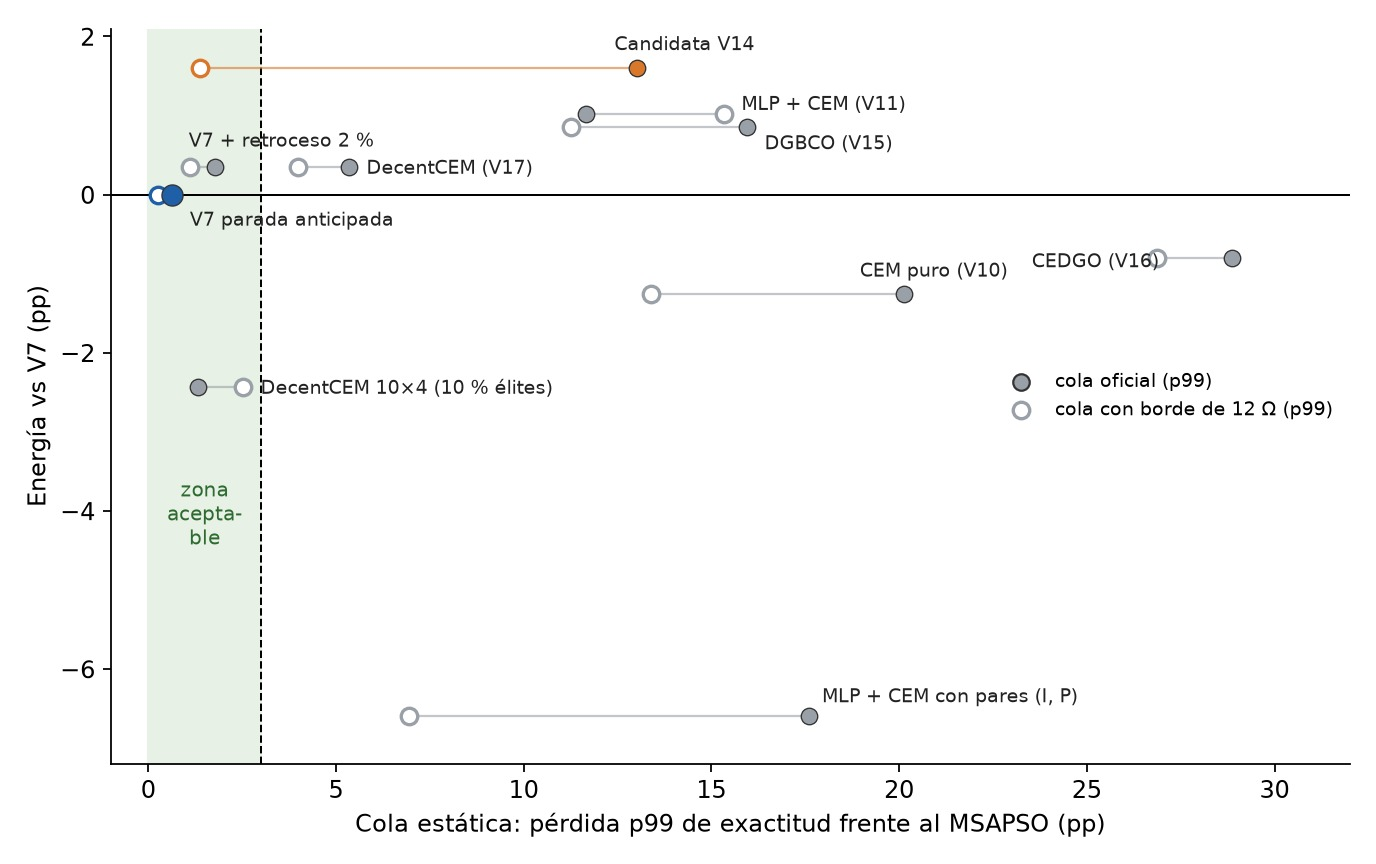
\includegraphics[width=0.78\linewidth]{figuras/fig3_energia_cola.jpg}
  \caption{Compromiso entre energía y cola. Eje horizontal: percentil 99 de la pérdida de exactitud estática frente al MSAPSO; el punto lleno es la cola oficial y el hueco la cola con borde de 12~$\Omega$. Eje vertical: diferencia de energía frente a la V7. La banda verde es el umbral previo (p99 $\leq$ 3~pp). Por encima de la línea de la V7 y dentro de la banda solo quedan la V7 + retroceso (cuya media de 0.53~pp excede el umbral en la cola oficial) y, con borde, la V14, que no cumple en el panel de 72 celdas.}
  \label{fig:cola}
\end{figure}

\begin{table}[H]
  \centering
  \caption{Cumplimiento de los criterios de aceptación, aplicados a cada método frente a la V7. (a) ventaja demostrable en prueba y confirmación; (c) pierde $>$ 3~pp en $\leq$ 10\,\% de escenarios; (d) cola con media $\leq$ 0.5~pp y p99 $\leq$ 3~pp, con la cola oficial y con la cola con borde de 12~$\Omega$ (entre paréntesis, media / p99; el desglose por panel solo se calculó para la V14). La condición (b) se evaluó por celdas en cada campaña (Anexo~A).}
  \label{tab:criterios}
  \scriptsize
  \setstretch{1}
  \begin{tabularx}{\linewidth}{@{}>{\raggedright\arraybackslash}p{2.2cm}>{\raggedright\arraybackslash}p{2.3cm}>{\raggedright\arraybackslash}p{1.25cm}>{\raggedright\arraybackslash}p{1.8cm}>{\raggedright\arraybackslash}p{2.2cm}>{\raggedright\arraybackslash}p{1.1cm}L@{}}
    \toprule
    \textbf{Método} & \textbf{(a) Ventaja} & \textbf{(c) Pierde $\leq$ 10\,\%} & \textbf{(d) Cola oficial} & \textbf{(d) Cola con borde} & \textbf{Brecha p99 oficial vs 3~pp} & \textbf{Lectura} \\
    \midrule
    V7 + retroceso 2\,\% & No (prueba: +0.08 [$-0.18$, 0.35]) & Sí (9\,\%) & No (media 0.53) & Sí (0.41 / 1.1) & $-1.2$ & Cola buena; el aporte no es demostrable en la prueba. \\
    Candidata V14 & Sí & Sí (7\,\%) & No (p99 13.0) & Panel base sí (1.4); no en todos (72 celdas: 6.4) & +10.0 & Más energía; alternativa con condiciones. Con 0.5~ms pierde 0.98~pp frente a la V7. \\
    MLP + CEM (V11) & Sí & No (18\,\%) & No (p99 11.7) & No (p99 15.3) & +8.7 & Requiere entrenamiento; $-3.3$~pp en casos de referencia del manuscrito. \\
    MLP + CEM con pares (I, P) & No (pierde $-6.59$) & No (40\,\%) & No (p99 17.6) & No (p99 6.9) & +14.6 & Las corrientes ayudan en estático, no en dinámica. \\
    DecentCEM (V17) & No (prueba: +0.43 [$-0.14$, 0.99]) & No (17\,\%) & No (p99 5.3) & No (p99 4.0) & +2.3 & Menor cola de los candidatos originales; pierde con espera de 0.5~ms. \\
    DecentCEM 10$\times$4 (10\,\% élites) & No (pierde $-2.44$) & No (28\,\%) & Sí (0.02 / 1.3) & Sí (0.07 / 2.5) & $-1.7$ & Cumple la cola, pero gasta $\approx$ 85 mediciones y pierde energía. \\
    DGBCO (V15) & Sí & No (16\,\%) & No (p99 15.9) & No (p99 11.3) & +12.9 & Gana poco con mala cola. \\
    CEM puro (V10) & No (pierde) & No (22\,\%) & No (p99 20.1) & No (p99 13.4) & +17.1 & Colapso de $\sigma$; sirve como refinador local. \\
    CEDGO (V16) & No (pierde) & No (22\,\%) & No (p99 28.9) & No (p99 26.9) & +25.9 & Sin espacio para los grupos con 40 mediciones. \\
    \bottomrule
  \end{tabularx}
\end{table}

\subsection{Ajuste, prueba y confirmación}
Ninguno de los métodos de búsqueda tiene pesos que se entrenen: su ``entrenamiento'' es el ajuste de parámetros (muestras, iteraciones, \textit{workers}, \% de élites), hecho solo con los escenarios 600--1199. La Tabla~\ref{tab:particiones} compara las tres particiones. Como no tienen la misma dificultad (en el ajuste todos, incluida la V7, le sacan más ventaja al MSAPSO), la comparación útil entre particiones es la columna \textit{vs V7}. No hay señales de sobreajuste: la V7 pasa de +3.58 a +2.98 y +2.78~pp frente al MSAPSO, el DecentCEM de +0.58 a +0.43 y +0.35~pp frente a la V7, y el DecentCEM 10$\times$4 de $-2.36$ a $-2.89$ y $-2.44$~pp, con intervalos que se traslapan.

\begin{table}[H]
  \centering
  \caption{Energía entregada por partición (\% de la máxima alcanzable) y diferencias en pp con IC 95\,\% (bootstrap pareado). Los parámetros se eligieron solo con el ajuste.}
  \label{tab:particiones}
  \scriptsize
  \setstretch{1}
  \setlength{\tabcolsep}{3pt}
  \resizebox{\linewidth}{!}{%
  \begin{tabular}{@{}llrrllr@{}}
    \toprule
    \textbf{Método} & \textbf{Partición} & \textbf{n} & \textbf{Energía} & \textbf{vs MSAPSO} & \textbf{vs V7} & \textbf{$>$3 pp} \\
    \midrule
    MSAPSO del paper & Ajuste (600--1199) & 600 & 84.26 & --- & $-3.58$ [$-4.27$, $-2.89$] & --- \\
     & Prueba (0--599) & 600 & 84.48 & --- & $-2.98$ [$-3.50$, $-2.47$] & --- \\
     & Confirmación (1200--2399) & 1\,200 & 84.60 & --- & $-2.78$ [$-3.18$, $-2.39$] & --- \\
    \addlinespace
    V7 parada anticipada & Ajuste & 600 & 87.84 & +3.58 [2.89, 4.27] & --- & 9\,\% \\
     & Prueba & 600 & 87.46 & +2.98 [2.47, 3.50] & --- & 7\,\% \\
     & Confirmación & 1\,200 & 87.38 & +2.78 [2.39, 3.18] & --- & 8\,\% \\
    \addlinespace
    DecentCEM (V17) & Ajuste & 600 & 88.42 & +4.16 [3.32, 4.97] & +0.58 [$-0.02$, 1.18] & 14\,\% \\
     & Prueba & 600 & 87.89 & +3.41 [2.66, 4.15] & +0.43 [$-0.14$, 0.99] & 14\,\% \\
     & Confirmación & 1\,200 & 87.73 & +3.13 [2.59, 3.65] & +0.35 [$-0.11$, 0.79] & 17\,\% \\
    \addlinespace
    DecentCEM 10$\times$4 (10\,\% élites) & Ajuste & 600 & 85.48 & +1.22 [0.44, 1.99] & $-2.36$ [$-3.00$, $-1.71$] & 27\,\% \\
     & Prueba & 600 & 84.57 & +0.09 [$-0.66$, 0.83] & $-2.89$ [$-3.53$, $-2.24$] & 31\,\% \\
     & Confirmación & 1\,200 & 84.94 & +0.35 [$-0.20$, 0.89] & $-2.44$ [$-2.92$, $-1.96$] & 28\,\% \\
    \bottomrule
  \end{tabular}}
\end{table}

El porcentaje de élites del DecentCEM 10$\times$4 se eligió del mismo modo (Tabla~\ref{tab:elites}). El 10\,\% (una élite de 10 muestras) es el que más energía da en el ajuste, y esa elección se sostiene en la confirmación. El \% de élites mueve la cola (p99 de 1.3~pp con 10\,\% a 4.6~pp con 100\,\%), no la energía: en la confirmación todos los porcentajes quedan entre $-2.86$ y $-2.44$~pp frente a la V7. Más muestras compran estabilidad a costa de energía: frente al DecentCEM original, la cola baja de 5.3 a 1.3~pp, pero la búsqueda sube de unas 40 a unas 85 mediciones. En la misma revisión se probaron 3 y 4 \textit{workers} con 4 a 9 muestras y 4 a 6 iteraciones. La cola con borde mejora (p99 de 1.0 a 1.4~pp con 6 muestras y $\approx$ 0.4~pp con 9 muestras y 3 élites), pero la energía frente a la V7 pasa a ser una pérdida demostrable de entre $-0.6$ y $-4.0$~pp (esta última con $\approx$ 110 mediciones).

\begin{table}[H]
  \centering
  \caption{DecentCEM 10$\times$4 según el porcentaje de élites (unas 85 mediciones por búsqueda en todos los casos). Cola: p99 oficial en 1\,000 curvas. Energía frente a la V7 en pp con IC 95\,\%. $\star$ = elegido en el ajuste.}
  \label{tab:elites}
  \scriptsize
  \setstretch{1}
  \begin{tabular}{@{}rrrlll@{}}
    \toprule
    \textbf{\% élites} & \textbf{Élites} & \textbf{p99} & \textbf{Ajuste vs V7} & \textbf{Prueba vs V7} & \textbf{Confirmación vs V7} \\
    \midrule
    \textbf{10 $\star$} & 1 & 1.33 & $-2.36$ [$-3.00$, $-1.71$] & $-2.89$ [$-3.53$, $-2.24$] & $-2.44$ [$-2.92$, $-1.96$] \\
    20 & 2 & 1.41 & $-2.63$ [$-3.27$, $-1.99$] & $-3.08$ [$-3.70$, $-2.44$] & $-2.73$ [$-3.22$, $-2.26$] \\
    30 & 3 & 1.55 & $-2.74$ [$-3.38$, $-2.10$] & $-3.10$ [$-3.76$, $-2.42$] & $-2.69$ [$-3.17$, $-2.23$] \\
    40 & 4 & 1.61 & $-2.68$ [$-3.35$, $-1.99$] & $-3.21$ [$-3.92$, $-2.53$] & $-2.66$ [$-3.14$, $-2.20$] \\
    50 & 5 & 1.86 & $-2.61$ [$-3.25$, $-2.00$] & $-2.99$ [$-3.60$, $-2.37$] & $-2.70$ [$-3.20$, $-2.23$] \\
    60 & 6 & 2.64 & $-2.62$ [$-3.26$, $-1.98$] & $-3.07$ [$-3.71$, $-2.41$] & $-2.79$ [$-3.28$, $-2.32$] \\
    70 & 7 & 3.23 & $-2.74$ [$-3.39$, $-2.07$] & $-3.07$ [$-3.72$, $-2.42$] & $-2.70$ [$-3.19$, $-2.23$] \\
    80 & 8 & 3.80 & $-2.79$ [$-3.43$, $-2.13$] & $-3.08$ [$-3.72$, $-2.41$] & $-2.79$ [$-3.29$, $-2.33$] \\
    90 & 9 & 4.21 & $-2.72$ [$-3.34$, $-2.09$] & $-2.92$ [$-3.56$, $-2.23$] & $-2.85$ [$-3.34$, $-2.38$] \\
    100 & 10 & 4.59 & $-2.79$ [$-3.42$, $-2.13$] & $-3.10$ [$-3.75$, $-2.44$] & $-2.86$ [$-3.35$, $-2.39$] \\
    \bottomrule
  \end{tabular}
\end{table}

\subsection{La cola: qué significa un mal caso}
La cola importa más que el promedio porque un error de búsqueda no es un error aislado: el controlador queda fijo en un punto equivocado hasta que la sombra cambie o la potencia varíe 5~W. La Figura~\ref{fig:peorcaso} muestra el peor caso de la candidata V14 frente a la V7 en la confirmación. La V14 se queda en un máximo local y entrega alrededor de 60\,\% del máximo alcanzable durante casi todo el escenario de 15~s, mientras que la V7 vuelve a buscar y se mantiene cerca del 100\,\%. En ese escenario la V14 entrega 34.6~pp menos de energía que la V7; en el promedio de los 1\,200 escenarios, en cambio, la V14 gana 1.6~pp. Un método con esa cola no es aceptable aunque su promedio sea mejor.

\begin{figure}[H]
  \centering
  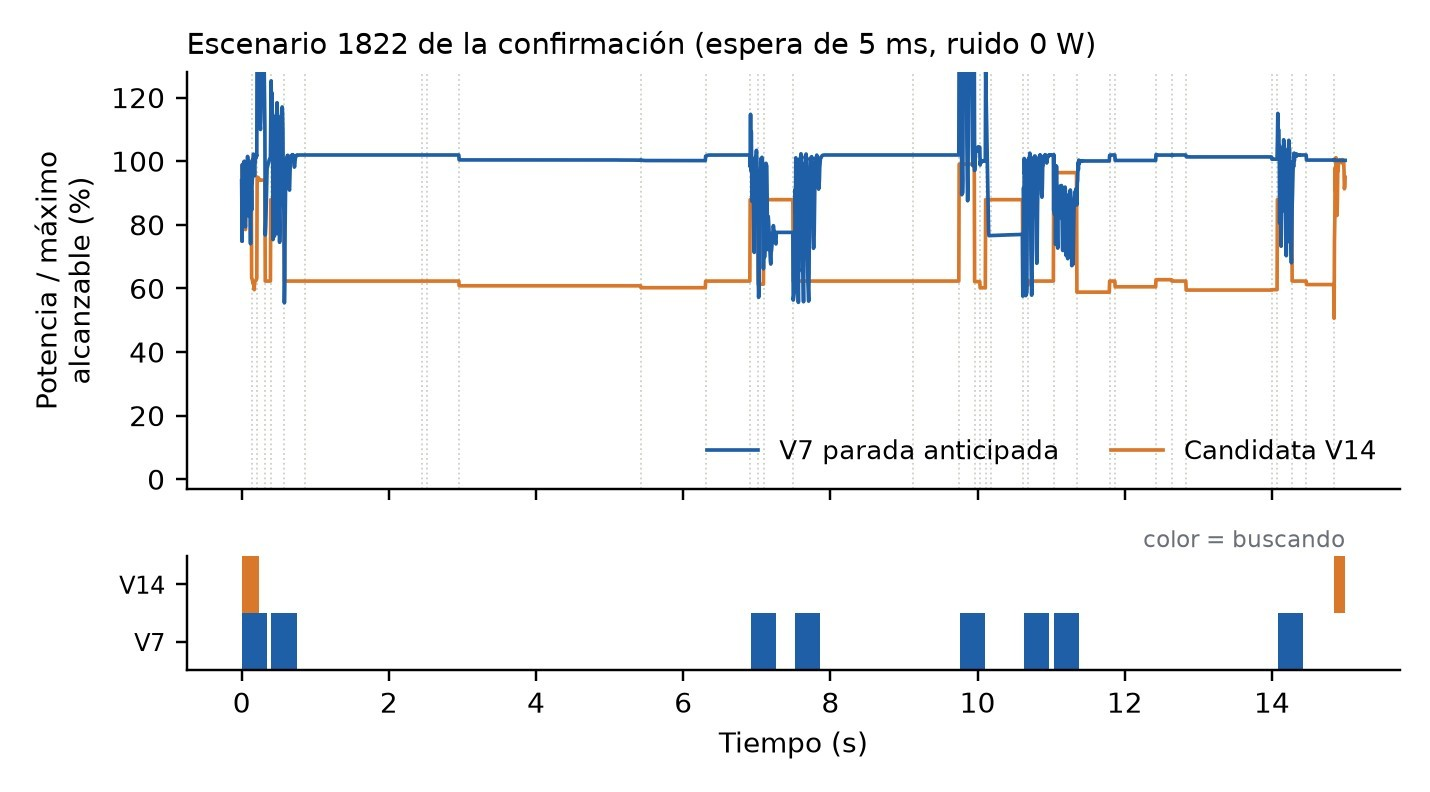
\includegraphics[width=0.82\linewidth]{figuras/fig4_peor_caso.jpg}
  \caption{Corrida real (simulador dinámico) del peor caso de la candidata V14 frente a la V7: escenario 1822 de la confirmación, espera de 5~ms, sin ruido. Arriba, potencia entregada como porcentaje del máximo alcanzable; las líneas punteadas son cambios de sombra. Abajo, los tramos en que cada método está buscando.}
  \label{fig:peorcaso}
\end{figure}

\subsection{Significado de los resultados en el contexto del proyecto}
Un punto porcentual de energía equivale a un 1\,\% de la energía que el arreglo podría entregar \textit{mientras dura la condición evaluada}. La ganancia de la V7 se concentra en sombra que cambia con frecuencia; en sombra estable no hay beneficio. Como ilustración, con supuestos hipotéticos (no medidos en una instalación): un arreglo de 1~kWp que produce 1\,500~kWh al año y pasa el 20\,\% de su energía en sombra cambiante ganaría $0.0278 \times 0.20 \times 1\,500 \approx$ \textbf{8~kWh por kWp al año ($\approx$ 0.6\,\%)}. Es una mejora modesta, coherente con un hallazgo previo (V6) de que el efecto anual neto de los híbridos era de décimas de punto. Su valor está en que se obtiene sin hardware adicional, sin entrenamiento y con menos cómputo (70 en lugar de 175 mediciones por búsqueda). El error de la V7 es pequeño y acotado: en 1\,000 curvas su pérdida máxima fue 0.97~pp frente al MSAPSO, y en el 8\,\% de los escenarios dinámicos pierde más de 3~pp, frente a 0\,\% del MSAPSO por construcción.

\subsection{Validez y amenazas}
Los resultados de prueba y confirmación coinciden (V7: +2.98 y +2.78~pp), lo que indica que no hay sobreajuste a los escenarios de ajuste (Tabla~\ref{tab:particiones}). Las amenazas principales son: la simulación y la reproducción propia del MSAPSO; que el régimen de 5~ms y la carga resistiva fija de 12~$\Omega$ limitan los puntos alcanzables; y que, al haber evaluado decenas de configuraciones sin corrección por comparaciones múltiples, los ganadores del ajuste están sesgados al alza. La revisión del asesor añadió tres amenazas de implementación. \textbf{(i)} Las partículas del MSAPSO y de la V7 se piden en 0.10 a 0.95 de $I_{sc}$, pero las más bajas caen en la zona que el Boost no alcanza y se miden cerca del borde; en la práctica el enjambre arranca con 4 o 5 posiciones distintas, no 7. Como la V7 se detiene hacia la pasada 10, un arranque mal repartido podría pesarle más que al MSAPSO (hipótesis no verificada). \textbf{(ii)} El CEM actualiza su gaussiana con la corriente pedida, no con la medida. \textbf{(iii)} En el DecentCEM la separación entre \textit{workers} se mide en la corriente pedida, así que dos \textit{workers} pueden medir el mismo punto físico en el borde. Por eso los intervalos relevantes son los de la confirmación. En DGBCO y CEDGO se fijaron con interpretaciones propias partes que los artículos no precisan (Moosavi et al., 2022; Tang et al., 2017), y el DGO se implementó con las ecuaciones tal como las reproduce el artículo de 2017, no con las del original.

% =====================================================================
\section{Implementación y operación}

\subsection{¿Se puede implementar o hay que retroceder?}
La V7 es implementable: no requiere datos de entrenamiento ni un modelo que mantener, usa unas 30 operaciones por pasada y es una modificación de una sola condición de salida sobre un algoritmo ya conocido. \textbf{No es necesario retroceder a la preparación de datos ni al modelado}. Lo que falta es validación fuera del simulador: la implementación del autor del MSAPSO, datos medidos y pruebas en hardware. Por eso la recomendación es de implementación \textbf{condicionada} a esas pruebas. Para la candidata V14 y los demás métodos sí hay que regresar a la fase de modelado. En la V14 el trabajo es más acotado de lo que sugería la cola oficial: con el borde de 12~$\Omega$ ya cumple la cola en el panel base, y falta corregirla en los paneles donde no cumple (72 celdas y 6 subcadenas), por ejemplo con más pasadas cuando el enjambre no converge, y repetir la evaluación completa.

\subsection{Requisitos operativos y responsables}
La Tabla~\ref{tab:requisitos} enumera lo necesario para operar la solución y propone un responsable por requisito, partiendo de la idea de Miller (2022) de que cada rol de interesado asume responsabilidades distintas. Al ser un proyecto académico, los roles concretos son una propuesta del equipo y son indicativos.

\begin{table}[H]
  \centering
  \caption{Requisitos para operar la V7 y responsables sugeridos.}
  \label{tab:requisitos}
  \footnotesize
  \setstretch{1}
  \begin{tabularx}{\linewidth}{@{}p{3.3cm}Lp{4.6cm}@{}}
    \toprule
    \textbf{Requisito} & \textbf{Qué se necesita} & \textbf{Responsable sugerido} \\
    \midrule
    Validación externa & Probar la V7 con la implementación del autor del MSAPSO y con datos medidos; confirmar si el convertidor real usa carga resistiva fija. & Asesor y equipo de investigación \\
    Caracterización del convertidor y del panel & Inductancia, carga, tiempo de espera mínimo útil, límites de corriente y de tensión. & Ingeniería de electrónica de potencia \\
    Implementación en el controlador & Pasar la V7 a firmware ($\approx$ 30 operaciones por pasada, sin entrenamiento), con tiempos de ejecución acotados. & Ingeniería de firmware \\
    Pruebas previas al despliegue & Banco de pruebas con hardware-in-the-loop; repetir los criterios (a)--(d) con el hardware real. & Responsable de pruebas y equipo \\
    Telemetría y almacenamiento & Registro de mediciones, reinicios y tiempo de búsqueda; canal seguro si hay nube. & Datos y TI \\
    Versionado y reversión & Entrega de versiones firmadas por actualización remota, con vuelta atrás ante una falla. & Firmware y TI \\
    Monitoreo y respuesta & Tablero, umbrales de alerta y procedimiento cuando se activan. & Operador de la instalación y equipo \\
    Gobernanza y comunicación & Aprobar criterios de aceptación y cambios; informar resultados y límites a los interesados. & Asesor académico \\
    \bottomrule
  \end{tabularx}
\end{table}

\subsection{Arquitectura de despliegue y proveedores}
El algoritmo de búsqueda debe ejecutarse \textbf{en el borde}, dentro del controlador del convertidor, porque cada medición dura milisegundos y el lazo no puede depender de una red. La nube solo tiene sentido para telemetría, monitoreo y entrega de versiones (Figura~\ref{fig:arquitectura}). Antes de desplegar cualquier versión se valida fuera de línea en el simulador y en un banco de pruebas.

\begin{figure}[H]
  \centering
  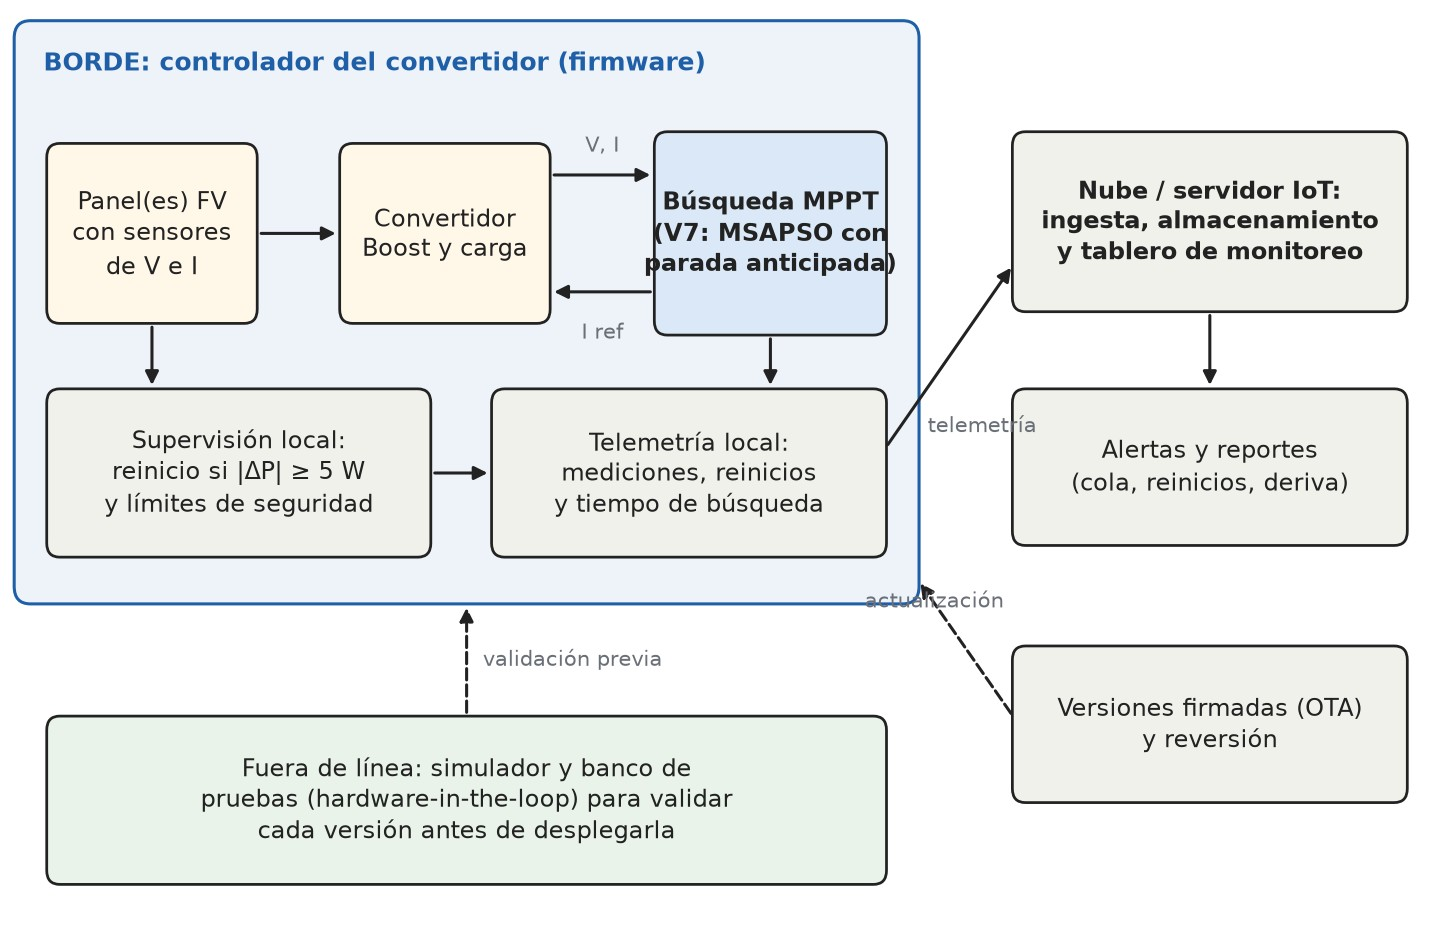
\includegraphics[width=0.82\linewidth]{figuras/fig5_arquitectura.jpg}
  \caption{Arquitectura de despliegue propuesta. El controlador (borde) ejecuta la búsqueda V7 y una supervisión local; la nube recibe telemetría, genera alertas y entrega versiones firmadas. Las flechas punteadas son flujos de validación y actualización.}
  \label{fig:arquitectura}
\end{figure}

Se revisaron los cuatro proveedores solicitados con el criterio de qué ofrecen para telemetría, monitoreo y actualizaciones de dispositivos (Tabla~\ref{tab:proveedores}). Dos de los servicios IoT gestionados de ese conjunto fueron retirados a finales de 2023, lo que pesa en la elección. La estructuración económica y de costos queda fuera del alcance de este artículo; su valoración corresponde a una etapa posterior, si el proyecto avanza hacia una implementación.

\begin{table}[H]
  \centering
  \caption{Valoración de proveedores para la capa de telemetría, monitoreo y actualización (no para el algoritmo, que corre en el borde).}
  \label{tab:proveedores}
  \footnotesize
  \setstretch{1}
  \begin{tabularx}{\linewidth}{@{}p{2.3cm}Lp{5.2cm}@{}}
    \toprule
    \textbf{Proveedor} & \textbf{Servicios relevantes} & \textbf{Valoración} \\
    \midrule
    AWS & IoT Greengrass v2 para despliegues y actualizaciones al borde; AWS IoT Core; CloudWatch y IoT Device Management para monitoreo (Amazon Web Services, s.\,f.). & Cubre telemetría, actualizaciones y monitoreo con servicios vigentes. \textbf{Opción recomendada} junto con Azure. \\
    Microsoft Azure & IoT Hub con gemelos de dispositivo; IoT Edge; Device Update for IoT Hub para actualizaciones y estado por dispositivo (Microsoft, s.\,f.). & Equivalente funcional a AWS; la elección depende de la infraestructura que ya tenga la institución. \\
    Google Cloud & Cloud IoT Core se retiró el 16 de agosto de 2023 (Hill, 2022). & Sin servicio IoT gestionado equivalente; habría que integrar servicios genéricos o de socios. \\
    IBM Watson & Watson IoT Platform se retiró sin reemplazo directo a finales de 2023 (Clark, 2022); Watson se orienta principalmente a servicios de IA, no al control en el borde. & No recomendada para esta capa. \\
    \bottomrule
  \end{tabularx}
\end{table}

En la fase académica puede bastar una alternativa mínima, con registro local en el controlador y un tablero sencillo, y dejar la nube para una etapa posterior si el proyecto escala.

\subsection{Monitoreo}
El monitoreo debe vigilar no solo la energía, sino sobre todo la cola y la salud del lazo (Tabla~\ref{tab:monitoreo}). Los umbrales numéricos deben calibrarse en el banco de pruebas, porque dependen del convertidor y del panel; las referencias de la tabla son las observadas en simulación.

\begin{table}[H]
  \centering
  \caption{Aspectos a supervisar durante la operación.}
  \label{tab:monitoreo}
  \footnotesize
  \setstretch{1}
  \begin{tabularx}{\linewidth}{@{}p{2.4cm}p{3.9cm}p{4.0cm}L@{}}
    \toprule
    \textbf{Aspecto} & \textbf{Indicador} & \textbf{Alerta (a calibrar en el banco de pruebas)} & \textbf{Motivo} \\
    \midrule
    Costo de búsqueda & Mediciones por búsqueda y fracción del tiempo buscando & Desvío frente a la línea base del simulador ($\approx$ 70 mediciones; 175 es el máximo) & Detecta enjambres que no convergen o reinicios excesivos \\
    Reinicios & Reinicios por hora & Aumento sostenido frente a la línea base & Señal de sombra turbulenta, ruido o falla de sensor \\
    Cola & Verificación periódica con un barrido completo (propuesta, no probada) & Potencia fija más de 3\,\% por debajo del barrido & Es el modo de falla que más pesa (Figura~\ref{fig:peorcaso}) \\
    Estabilidad tras fijar & $|\Delta P|$ entre ventanas con la corriente fija & Cercanía al umbral de 5~W & Anticipa reinicios innecesarios \\
    Sensores y ruido & Dispersión de las lecturas & Ruido por encima del rango validado (1--2~W) & Con ruido alto la regla de parada se vuelve poco confiable \\
    Deriva del sistema & Cambios de $I_{sc}$, $V_{oc}$ y respuesta del convertidor & Fuera del rango de caracterización & Envejecimiento o suciedad del panel; reajuste del tiempo de espera \\
    Versión y salud del lazo & Versión de firmware, errores y saltos de comunicación & Cualquier discrepancia con la versión validada & Trazabilidad y reversión \\
    \bottomrule
  \end{tabularx}
\end{table}

\subsection{Decisiones recomendadas a partir de los hallazgos}
\begin{itemize}[leftmargin=1.5em, itemsep=2pt]
  \item \textbf{Adoptar la V7} como candidata a implementación, condicionada a la validación en hardware descrita en la Tabla~\ref{tab:requisitos}.
  \item \textbf{Mantener la candidata V14 como alternativa con condiciones}: con el borde de 12~$\Omega$ cumple la cola en el panel base, pero no en todos los paneles. No adoptarla hasta que cumpla en cada panel tras un respaldo que la acote.
  \item \textbf{Aplicar el retroceso del 2\,\%} solo después de validarlo en hardware: aporta +0.35~pp a la V7 pero eleva su pérdida estática media de 0.05 a 0.53~pp, por encima del umbral de 0.5~pp.
  \item \textbf{Descartar los métodos poblacionales} (CEM puro, DGBCO, CEDGO) con presupuestos de 40 a 70 mediciones, y no invertir más en variantes de los mismos.
  \item \textbf{No seguir aumentando muestras, iteraciones o \textit{workers} del DecentCEM}: el DecentCEM 10$\times$4 cumple la cola, pero con unas 85 mediciones pierde 2.44~pp frente a la V7.
\end{itemize}

% =====================================================================
\section{Conclusiones clave}

\subsection{Hallazgos principales}
\begin{itemize}[leftmargin=1.5em, itemsep=2pt]
  \item El MSAPSO ya está cerca del techo de exactitud: ninguna de las 18 versiones lo superó en exactitud final. El margen está en el costo de búsqueda y en la energía con sombra cambiante.
  \item La mejora que sobrevivió a todas las pruebas fue la más simple: \textbf{detener el enjambre cuando se agrupa} (V7). Ahorra 60\,\% de las mediciones, gana +2.78~pp de energía [2.39, 3.18] en la confirmación y mantiene una cola estática de p99 = 0.64~pp.
  \item Evaluar con un baseline fiel, energía dinámica, escenarios frescos y la cola cambió las conclusiones: varios éxitos iniciales desaparecieron y la cola resultó más decisiva que el promedio.
  \item Un margen fijo del 2\,\% de la corriente explica la ventaja dinámica del MLP y aporta +0.90~pp a la candidata V14: conviene probar un control sin aprendizaje antes de entrenar un modelo.
  \item Con 40 a 70 mediciones, los métodos poblacionales no tienen espacio para separarse de un enjambre fijo con parada anticipada. Refinar cada pico por separado (DecentCEM) reduce mucho la cola de la V14, pero no basta para igualar a la V7. Con más muestras (DecentCEM 10$\times$4, 10\,\% de élites) la cola cumple el umbral, pero el costo de búsqueda borra la ventaja de energía ($-2.44$~pp).
  \item La forma de medir la cola importa. Con el borde de 12~$\Omega$ la V14 cumple en el panel base (p99 1.4~pp) pero no en todos los paneles (hasta 6.4~pp); la cola debe evaluarse con el convertidor real y por panel.
  \item Darle al MLP las corrientes medidas, además de las potencias, baja su cola con borde de 15.3 a 6.9~pp, pero en dinámica pierde $-6.59$~pp frente a la V7: la red recibe pares rezagados que no vio al entrenar.
\end{itemize}

\subsection{Limitaciones}
\begin{itemize}[leftmargin=1.5em, itemsep=2pt]
  \item Solo simulación, con una reproducción propia del MSAPSO a partir de una versión borrador; sin datos medidos ni hardware.
  \item Carga resistiva fija de 12~$\Omega$ y régimen de 5~ms; a 0.5~ms el convertidor no sigue las referencias y la ventaja de los métodos cortos se reduce o se invierte.
  \item Interpretaciones propias en DGBCO y CEDGO; muchas configuraciones evaluadas sin corrección por comparaciones múltiples.
  \item El primer muestreo del MSAPSO y de la V7 cae en parte en la zona inalcanzable; los MLP se entrenaron con barridos estáticos, distintos de lo que mide el convertidor en operación.
  \item La condición de cumplir la cola en cada panel se añadió después de las campañas y solo se evaluó para la V14.
  \item La traducción a kWh por año usa supuestos ilustrativos, no mediciones de una instalación.
\end{itemize}

\subsection{Trabajo futuro}
\begin{itemize}[leftmargin=1.5em, itemsep=2pt]
  \item Validar la V7 con la implementación del autor, con datos medidos y en un banco con hardware-in-the-loop (primer paso para implementarla).
  \item Diseñar un respaldo contra la cola de la candidata V14 en los paneles donde no cumple (72 celdas y 6 subcadenas) y repetir la campaña con el mismo protocolo.
  \item Sembrar las partículas del MSAPSO y de la V7 solo dentro de la zona alcanzable y medir su efecto.
  \item Evaluar el retroceso del 2\,\% y el DecentCEM combinados en dinámica (no se probó), y entrenar el MLP con pares (I, P) con barridos del simulador dinámico, para que vea en el entrenamiento las corrientes rezagadas que mide en operación.
  \item Probar el entrenamiento de la red muestreando sus pesos (neuroevolución con CEM), que no se evaluó, y la memoria de patrones con sombras realmente recurrentes.
\end{itemize}

% --- Declaración de uso de IA (antes de las referencias) ---
\section*{Declaración de uso de inteligencia artificial}
Se utilizó Claude (Sonnet 5.5) (Anthropic, 2026) a lo largo del proyecto como asistente de investigación y desarrollo: para implementar y ejecutar el simulador y las campañas de simulación (V2 a V19), explorar alternativas (aprendizaje por refuerzo, redes neuronales, CEM, DGBCO, DGO/CEDGO y DecentCEM, incluidas las variantes de la revisión del asesor), investigar y verificar fuentes, analizar los resultados y generar las figuras y la demostración interactiva. El borrador de este artículo se redactó con su apoyo y fue revisado, editado y asumido por los autores. La responsabilidad final sobre el contenido entregado recae en los autores.

% --- Referencias (APA 7) ---
\section*{Referencias}
\begingroup
\setstretch{1}\small\sloppy
\setlength{\parindent}{-1.27cm}\setlength{\leftskip}{1.27cm}\setlength{\parskip}{5pt}

\noindent\hspace*{-1.27cm}Amazon Web Services. (s.\,f.). \textit{Update the AWS IoT Greengrass Core software (OTA)}. AWS IoT Greengrass Version 2 Developer Guide. \url{https://docs.aws.amazon.com/greengrass/v2/developerguide/update-greengrass-core-v2.html}

Anthropic. (2026). \textit{Claude (Sonnet 5.5)} [Modelo de lenguaje grande]. \url{https://claude.ai}

Clark, L. (2022, 15 de noviembre). IBM to fire Watson IoT Platform from its cloud. \textit{The Register}. \url{https://www.theregister.com/2022/11/15/ibm_set_to_retire_watson/}

Efron, B., y Tibshirani, R. J. (1993). \textit{An introduction to the bootstrap}. Chapman \& Hall.

Hill, K. (2022, 16 de agosto). Google Cloud to shut down IoT Core service next year. \textit{RCR Wireless News}. \url{https://www.rcrwireless.com/20220816/internet-of-things/google-cloud-to-shut-down-iot-core-service-next-year}

\textit{Hybrid MPPT with deterministic PSO and Super-Twisting: Minimum-time tracking under complex partial shading}. (2025). [Manuscrito no publicado, versión borrador proporcionada por el asesor].

Kennedy, J., y Eberhart, R. (1995). Particle swarm optimization. En \textit{Proceedings of ICNN'95 -- International Conference on Neural Networks} (Vol.~4, pp.~1942--1948). IEEE. \url{https://doi.org/10.1109/ICNN.1995.488968}

Korolov, M. (2022, 7 de septiembre). Measuring the business impact of AI. \textit{CIO}. \url{https://www.cio.com/article/405620/measuring-the-business-impact-of-ai.html}

Levant, A. (2003). Higher-order sliding modes, differentiation and output-feedback control. \textit{International Journal of Control, 76}(9--10), 924--941. \url{https://doi.org/10.1080/0020717031000099029}

Microsoft. (s.\,f.). \textit{Understand Device Update for IoT Hub}. Microsoft Learn. \url{https://learn.microsoft.com/azure/iot-hub-device-update/understand-device-update}

Miller, G. (2022). Stakeholder roles in artificial intelligence projects. \textit{Project Leadership and Society, 3}, 100068. \url{https://doi.org/10.1016/j.plas.2022.100068}

Moosavi, S. K. R., Mansoor, M., Zafar, M. H., Khan, N. M., Mirza, A. F., y Akhtar, N. (2022). Highly efficient maximum power point tracking control technique for PV system under dynamic operating conditions. \textit{Energy Reports, 8}, 13529--13543. \url{https://doi.org/10.1016/j.egyr.2022.10.011}

Moss, R. J. (2020). \textit{Cross-entropy method variants for optimization} (arXiv:2009.09043). arXiv. \url{https://arxiv.org/abs/2009.09043}

Rubinstein, R. Y., y Kroese, D. P. (2004). \textit{The cross-entropy method: A unified approach to combinatorial optimization, Monte-Carlo simulation, and machine learning}. Springer.

Schulman, J., Wolski, F., Dhariwal, P., Radford, A., y Klimov, O. (2017). \textit{Proximal policy optimization algorithms} (arXiv:1707.06347). arXiv. \url{https://arxiv.org/abs/1707.06347}

Tang, R., Fong, S., Dey, N., Wong, R. K., y Mohammed, S. (2017). Cross entropy method based hybridization of dynamic group optimization algorithm. \textit{Entropy, 19}(10), 533. \url{https://doi.org/10.3390/e19100533}

Williams, R. J. (1992). Simple statistical gradient-following algorithms for connectionist reinforcement learning. \textit{Machine Learning, 8}(3--4), 229--256. \url{https://doi.org/10.1007/BF00992696}

Zhang, Z., Jin, J., Jagersand, M., Luo, J., y Schuurmans, D. (2022). \textit{A simple decentralized cross-entropy method} (arXiv:2212.08235). arXiv. \url{https://arxiv.org/abs/2212.08235}

\endgroup


% --- Anexos (en página nueva; \appendix cambia la numeración a A, B, ...) ---
\clearpage
\appendix
\renewcommand{\thesection}{\Alph{section}}
\titleformat{\section}{\Large\bfseries}{Anexo \thesection.}{0.6em}{}

\section{Cifras del artículo y su fuente}
Cada cifra decisiva del cuerpo del artículo, con el archivo del que proviene, para contrastarla con los notebooks y reportes entregados.

\begin{table}[H]
  \centering
  \caption{Cifras decisivas y fuentes. Carpeta base: Proyecto Integrador (versiones V2--V19).}
  \label{tab:cifras}
  \footnotesize
  \setstretch{1}
  \begin{tabularx}{\linewidth}{@{}p{4.3cm}p{4.0cm}L@{}}
    \toprule
    \textbf{Cifra} & \textbf{Valor} & \textbf{Fuente} \\
    \midrule
    Mediciones por búsqueda: MSAPSO / V7 & 175 / 70 & Paneles\_V7/Reporte\_Corrida\_V7.pdf; V19/resultados\_V19/est\_V19.json \\
    Energía MSAPSO / V7 (confirmación) & 84.60\,\% / 87.38\,\% & Paneles\_V19/resultados\_V19/dyn\_V19.json (índices 1200--2399) \\
    V7 $-$ MSAPSO (confirmación / prueba) & +2.78 [2.39, 3.18] / +2.98 [2.47, 3.50] pp & ídem (bootstrap pareado, 3\,000 remuestreos) \\
    V7 en 2\,400 escenarios (campaña V7) & +3.0 [2.7, 3.3] pp; pierde $>$ 3~pp en 8\,\% & Paneles\_V7/Reporte\_Corrida\_V7.pdf; Resumen\_Consolidado\_V2-V16 \\
    Cola estática V7 (1\,000 curvas) & media 0.053; p99 0.64; máx. 0.97~pp & Paneles\_V19/resultados\_V19/est\_V19.json \\
    Candidata V14 $-$ V7 (confirmación) & +1.60 [1.24, 1.96] pp; cola p99 13.0, máx. 23.0 & dyn\_V19.json; est\_V19.json; Paneles\_V14/README.md \\
    Candidata V14 $-$ V7 (2\,400 escenarios) & +1.54 [1.31, 1.78] pp & Paneles\_V14/README.md \\
    Retroceso 2\,\%: aporte a V14 / a V7 & +0.90 [0.65, 1.16] / +0.35~pp & Paneles\_V13/README.md; V19/dyn\_V19.json \\
    DecentCEM $-$ V7 (prueba / confirmación) & +0.43 [$-0.14$, 0.99] / +0.35 [$-0.11$, 0.79]~pp & Paneles\_V17/resultados\_V17/dc\_test\_V17.txt, dc\_conf\_V17.txt \\
    DecentCEM: cola estática & media 0.245; p99 5.34; máx. 7.64~pp & Paneles\_V17/resultados\_V17/dc\_S\_V17.txt \\
    MLP con corrientes (puntos aleatorios) & +0.74 [0.55, 0.92] y +0.64 [0.46, 0.82]~pp & Paneles\_V18/resultados\_V18/mlp\_pares\_V18.txt \\
    Reproducción de campañas anteriores & diferencia 0.0 en V13, V15, V16 y V17 & Paneles\_V19/campana\_V19.py (comprobación al final de ``dyn'') \\
    \addlinespace
    \multicolumn{3}{@{}l}{\textit{Revisión del asesor (cifras del simulador fusionado; Anexo~C)}} \\
    Cola con borde de 12~$\Omega$ (todos los métodos) & V7: 0.03 / 0.27 / 0.64~pp; V14: 0.45 / 1.38 / 6.31~pp & \nolinkurl{Simulador/Simulador_Comparativo_MPPT/cola_con_borde.py}; pestaña Resultados del simulador \\
    V14 con borde: otras 1\,000 curvas y por panel & 0.45 / 2.3 / 9.1~pp; p99 por panel 72c 6.4 y 3.8, 60c-11A 1.2 y 3.6, 36c 0.8 y 1.2, 96c 0.6 y 0.6 & Ficha de la V14 en el simulador \\
    MLP + CEM con pares (I, P) $-$ V7 (confirmación) & $-6.59$ [$-7.36$, $-5.82$] pp; cola 17.6 oficial / 6.9 con borde & \nolinkurl{Simulador 2/Simulador_Comparativo_MPPT/campana.py}; pestaña Resultados \\
    DecentCEM 10$\times$4 (10\,\% élites) $-$ V7 & ajuste $-2.36$, prueba $-2.89$, confirmación $-2.44$ [$-2.92$, $-1.96$] pp & \nolinkurl{Simulador 2/Simulador_Comparativo_MPPT/campana.py} (dyn con la opción de ajuste); tabla de particiones del simulador \\
    DecentCEM 10$\times$4 (10\,\% élites): cola & oficial 0.02 / 1.33 / 7.22~pp; con borde 0.07 / 2.52 / 9.43~pp; 85 mediciones & campana.py (est) y cola\_con\_borde.py, método \nolinkurl{decent_n10_e10} \\
    \bottomrule
  \end{tabularx}
\end{table}

\section{Configuración de los once métodos}

\begin{table}[H]
  \centering
  \caption{Configuración congelada de cada método (la de su propia campaña; sin reajustes). b = retroceso de corriente; med. = mediciones.}
  \label{tab:config}
  \footnotesize
  \setstretch{1}
  \begin{tabularx}{\linewidth}{@{}p{3.0cm}L@{}}
    \toprule
    \textbf{Método} & \textbf{Configuración} \\
    \midrule
    MSAPSO del paper & 7 partículas $I_{sc}\cdot$[0.95, 0.80, 0.65, 0.50, 0.30, 0.15, 0.10]; $\beta$ de 0.1 a 0.95; 25 pasadas (175 med.); reinicio si $|\Delta P| \geq 5$~W; b = 0. \\
    V7 & Igual, con parada cuando std($x$)/$I_{sc}$ $<$ 0.02 (mínimo 3 pasadas); b = 0. \\
    V7 + retroceso & V7 con b = 0.02. \\
    CEM puro (V10) & $\mu_0$ = 0.5, $\sigma_0$ = 0.3, 10 candidatos, 3 élites, $\alpha$ = 0.7, parada $\sigma$ $<$ 0.01, hasta 25 iteraciones; b = 0. \\
    MLP + CEM (V11) & Barrido de 7 puntos; MLP (64, 64) entrenado con 30\,000 sombras predice $x^*$; CEM (7 candidatos, 2 élites, $\alpha$ = 0.7, $\sigma_0$ = 0.1, parada $\sigma$ $<$ 0.005); b = 0. \\
    Candidata V14 & 3 pasadas de MSAPSO ($\beta$ comprimida) + CEM (7 candidatos, 2 élites, $\alpha$ = 0.7, $\sigma_0$ = 0.03, parada $\sigma$ $<$ 0.005); b = 0.02. \\
    DGBCO (V15) & 4 agentes $\times$ 10 iteraciones (40 med.), inicialización tipo MSAPSO, 70\,\% exploración / 30\,\% explotación; b = 0.02. \\
    CEDGO (V16) & 8 individuos $\times$ 5 generaciones (40 med.), 2 grupos, operador CE, vuelo de Lévy, tiempo de vida 3; b = 0.02. \\
    DecentCEM (V17) & Barrido de 10 puntos; élites separadas por más de 0.15 se vuelven \textit{workers}; $\sigma$ fija 0.03; 4 muestras $\times$ 4 iteraciones por \textit{worker}; b = 0. \\
    MLP + CEM con pares (I, P) & Barrido de 7 puntos; MLP (64, 64) que recibe los pares (corriente medida, potencia), entrenado con 30\,000 sombras (semilla 1111) y con cada corriente por debajo del borde de 12~$\Omega$ medida en el borde; etiqueta = corriente del máximo teórico / $I_{sc}$; CEM idéntico al de la V11; b = 0. \\
    DecentCEM 10$\times$4 & Como la V17, con 10 muestras por iteración, 4 iteraciones y hasta 3 \textit{workers}; élites = 10\,\% de las muestras (1 élite), elegido en el ajuste entre 10 y 100\,\%; 10 + \textit{workers} $\times$ 40 mediciones ($\approx$ 85 en promedio); b = 0. \\
    \bottomrule
  \end{tabularx}
\end{table}

\section{Reproducibilidad y demostración interactiva}
El código, los reportes de cada versión y los resultados por escenario están en el repositorio del proyecto (https://github.com/pedro-mrqz/msapso-mppt). La demostración interactiva es un solo archivo HTML (Simulador 2/Presentacion/simulador\_fusionado\_particiones.html). Reproduce, medición por medición, las corridas reales de los once métodos sobre los cuatro casos de referencia del manuscrito, con cualquier combinación de tiempo de espera y ruido, y con el porcentaje de élites del DecentCEM 10$\times$4 seleccionable (10\,\% por defecto). Incluye una ficha descriptiva de cada método y una pestaña de resultados con las cifras de la Tabla~\ref{tab:metodos} (cola oficial y con borde) y las tablas de particiones y de \% de élites (Tablas~\ref{tab:particiones} y~\ref{tab:elites}). No incluye escenarios con cambios de sombra, así que el peor caso de la Figura~\ref{fig:peorcaso} no se puede reproducir en él.

\end{document}
